\section{Problem 10}
The min-max composition of fuzzy relations is a method for combining two fuzzy relations to produce a new fuzzy relation. The process is somewhat analogous to matrix multiplication in linear algebra but uses the "min" and "max" operations instead of multiplication and addition. \\
Given two fuzzy relations $R1$ and $R2$, with membership functions $\mu_{\tilde{R1}}(x,y)$ and $\mu_{\tilde{R2}}(y,z)$ respectively, the min-max composition $R = R1 \circ R2 $ has a membership function defined for each pair $(x,z)$ by:
\begin{equation}
	\mu_R(x, z) = \max_{y} \min(\mu_{R1}(x, y), \mu_{R2}(y, z)
\end{equation}

In order to gain a deeper understanding, , we will analyse the expression
\begin{itemize}
	\item $\min(\mu_{R1}(x, y), \mu_{R2}(y, z)$: For a fixed $x$ and $z$, and for each intermediate value of $y$, we must calculate the minimum membership value between 
	$\mu_{\tilde{R1}}(x,y)$ and $\mu_{\tilde{R2}}(y,z)$ . This minimum value represents the strongest constraint on the relationship between $x$ and $z$ via the intermediary $y$.
	\item $\max_{y} $: Select the maximum value out of all these minimum values as the membership degree for the pair $(x,z)$ in the relation $R$.
\end{itemize}

Now, let's analyze the exponential terms within the membership functions. We have:
\begin{align}
	\mu_{\tilde{R1}}(x,y) = e^{-k(x - y)^2}, \quad \text{for } k \geq 1 \\
	\mu_{\tilde{R2}}(y,z) = e^{-k(y - z)^2}, \quad \text{for } k \geq 1
\end{align}
The exponential function $e^{-k(w)^2}$  is a Gaussian function that has its maximum value when 
$w=0$ and decreases as $w$ moves away from $0$ in either direction. This means that for a fixed 
$x$ and $z$, the membership values $\mu_{\tilde{R1}}(x,y)$ and $\mu_{\tilde{R2}}(y,z)$ will be higher when $y$ is close to $x$ and $z$ respectively, because the terms $(x-y)^2$ and $(y-z)^2$ will be smaller, making the exponent closer to $0$.\\

When we take the minimum of these two membership values, we are essentially looking for the point where the overlap between the two functions is the greatest, since the minimum value is dominated by the smaller of the two membership degrees.
\\

In other words, since the membership functions involve an exponential function of a squared term, the minima will occur where the arguments of the exponential functions are closest to each other, that is, when $(x-y)^2$ and $(y-z)^2$
are minimal.
\\

Graphically, we can represent the membership functions $\mu_{R1}$ and $\mu_{R2}$ as surfaces over $x-y$ and $y-z$ planes, respectively. The composition $\mu_R$ would be a new surface over the $x-z$ plane, which is derived from the "peaks" of the minimum values between the two original surfaces for every $x$ and $z$. We will assume a value for $k$ to proceed with the calculation. Let's set $k=1$ for simplicity. We will first define the membership functions and then compute the max-min composition for a range of 
$x$ and 
$z$ values.

\begin{figure}[H]
	\centering
	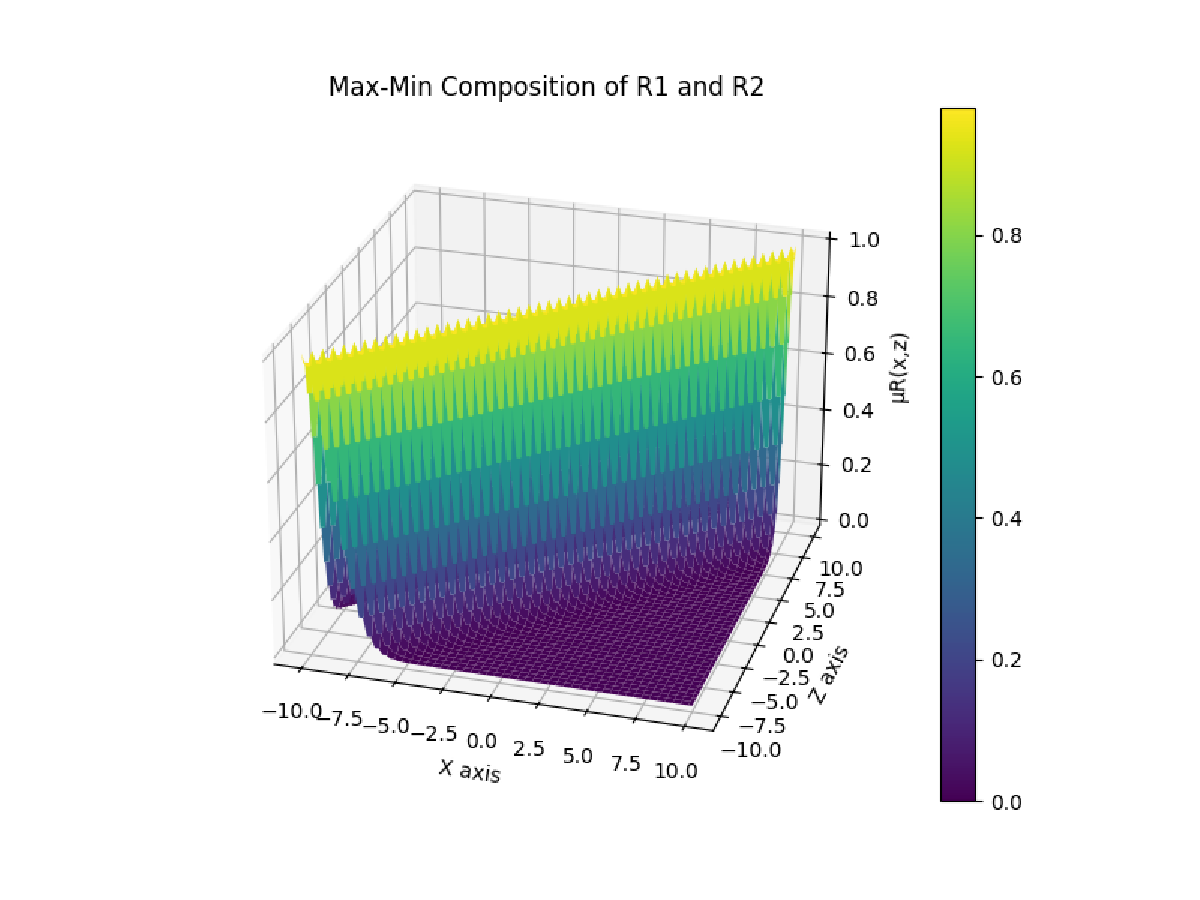
\includegraphics[width=0.8\textwidth]{../Problem 10/minmax_plot.pdf}
	\caption{Max-Min Composition of Fuzzy Relations R1 and R2}
\end{figure}
The 3D plot above shows the Max-Min composition of the fuzzy relations $R_1$ and $R_2$ over the range of $x$ and $z$ values. The surface represents the degree of membership in the composite relation for each pair $(x, z)$, calculated as the maximum of the minimum values of $\mu_{\tilde{R1}}(x,y)$ and $\mu_{\tilde{R2}}(y,z)$  across all posible values of $y$. The height of the surface at any point indicates the strength of the relation between $x$ and $z$ in the composite relation $R$.